% Author        : PokMan Ho
% Script        : 20200515_result.tex
% Desc          : MRes progress report tex
% Input         : none
% Output        : pdf report in same directory
% Arguments     : 0
% Date          : May 2020

\documentclass[a4paper,11pt]{article}
\usepackage[margin=2cm]{geometry}
\usepackage[english]{babel}
\usepackage{graphicx, hyperref, longtable, amsmath, amssymb}
\graphicspath{{figure/}{figure/}}

\hypersetup{
	colorlinks=true,
	linkcolor=blue,
	filecolor=blue,      
	urlcolor=blue,
	citecolor=blue
}

\title{R vs py3 engines in Julia-lang kernel}
\author{PokMan Ho}

\begin{document}
    \maketitle
    \section{Summary}
    \begin{itemize}
        \item most discrepancies fixed -- this is sourced from a dumb mistake on parameter arrangement
        \item situations' equilibrium position are mostly coexisting, with a small portion of phytoplankton-dominating situations (see pie charts below)
        \item R \& py3 integration engines now mostly agreeing on each other, exception samples listed below
        \item initial carbon densities alter a tiny fraction of situations
    \end{itemize}
    
    \section{document links}
    \begin{itemize}
        \item third-party calculation using Google  \href{https://docs.google.com/spreadsheets/d/1k4eZ2qmefPx8dAj6BVPFUE00JBayk8zqMAfbH60slB8/edit#gid=939440998}{spreadsheet} tab ``analytical"
        \item function bin scripts in \href{https://github.com/ph-u/Project/blob/master/code/func.R}{R-lang} and \href{https://github.com/ph-u/Project/blob/master/code/func.jl}{Julia-lang}, which are functionally-identical
        \item Jupyter notebooks doing the same thing using \href{https://nbviewer.jupyter.org/github/ph-u/Project/blob/master/sandbox/cpb_0514_r.ipynb}{R-lang} and \href{https://nbviewer.jupyter.org/github/ph-u/Project/blob/master/sandbox/cpb_0514_jp.ipynb}{Julia-lang}
    \end{itemize}
    
    \section{Descriptions for chosen parameter set samples}
    Larger differences between results were observed in section:
    \begin{center}
        \begin{tabular}{cc|r}\hline
            section & iniPop & reason\\\hline
            3.1 & $10^{-12}$ & final result diff\\
            4.1 & $10^{-8}$ & carbon density time series trace diff\\
            5.1 & $10^{-12}$ & R model crashed\\\hline
        \end{tabular}
    \end{center}
    
    Equilibrium solutions were listed below:
    \begin{center}
        \begin{tabular}{c|ccc}\hline
            Sol & C & P & B\\\hline
            (1) & 0 & 0 & 0\\
            (2) & $\frac{m_B}{e_{BR}e_B g_B}$ & 0 & $\frac{x}{g_B(e_{BR} - 1)}$\\
            (3) & $\frac{e_P(e_{PR}g_P)^2}{a_P x}$ & $\frac{e_{PR}e_Pg_P}{a_P}$ & 0\\
            (4) & $\frac{m_B}{e_{BR}e_B g_B}$ & $\frac{e_{PR}e_P g_P}{a_P}$ & $\frac{a_P m_B x - e_{BR}e_B g_B e_P(e_{PR}g_P)^2}{a_P m_B g_B(e_{BR}-1)}$\\\hline
        \end{tabular}
    \end{center}
    
    \section{distributions from parameter space scanning: 1234321 situations}
    \begin{itemize}
        \item $x$: seq(0:1, by=.01)
        \item $e_{PR}$: .875
        \item $e_P$: .63
        \item $g_P$: seq(0.259:0.556, by=(.556-.259)/10)
        \item $a_P$: seq(0.001:0.400, by=(.4-.001)/10)
        \item $e_{BR}$: .6
        \item $e_B$: .55
        \item $g_B$: seq(0.707:9.010, by=(9.01-.707)/100)
        \item $m_B$: .14
    \end{itemize}
    solution type 0 = numerical solution too far ($>$=10 gC/m$^3$) from any analytical solutions\\
    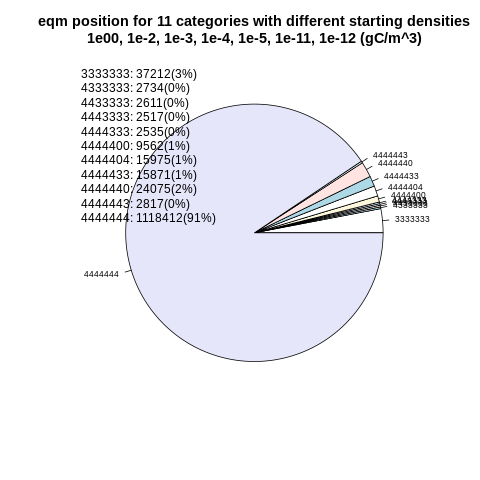
\includegraphics[width=.6\linewidth]{sandbox/graph/eqmPoSum.png}
    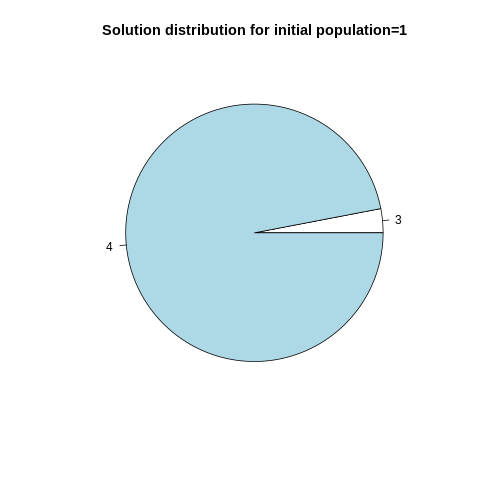
\includegraphics[width=.3\linewidth]{sandbox/graph/1e-0.png}\\
    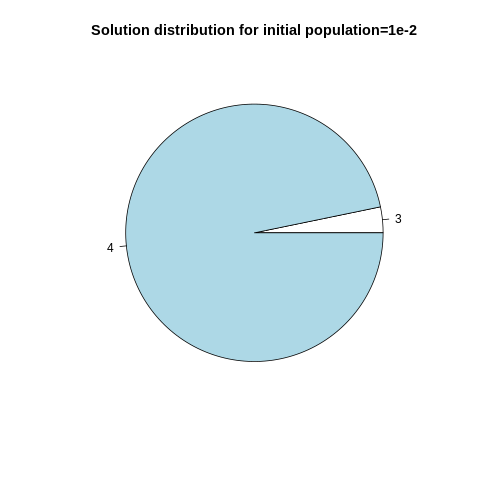
\includegraphics[width=.3\linewidth]{sandbox/graph/1e-2.png}
    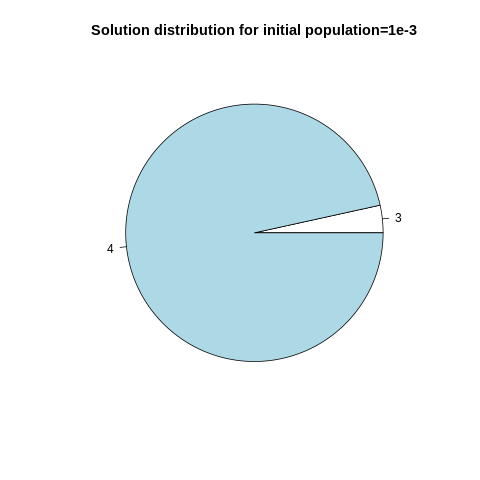
\includegraphics[width=.3\linewidth]{sandbox/graph/1e-3.png}
    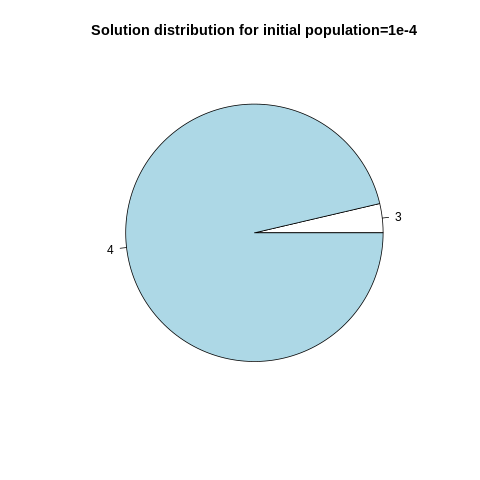
\includegraphics[width=.3\linewidth]{sandbox/graph/1e-4.png}\\
    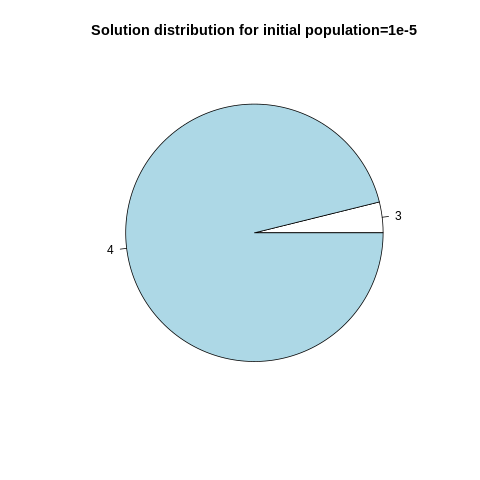
\includegraphics[width=.3\linewidth]{sandbox/graph/1e-5.png}
    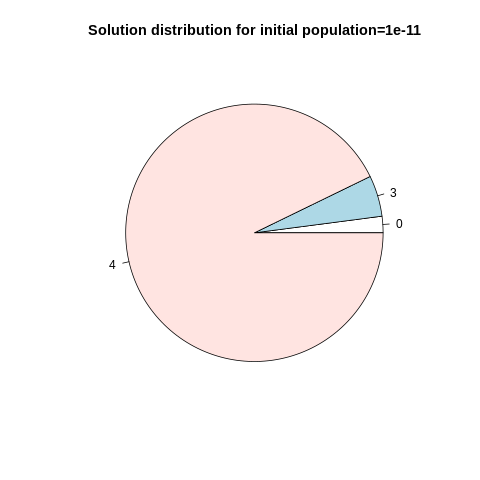
\includegraphics[width=.3\linewidth]{sandbox/graph/1e-11.png}
    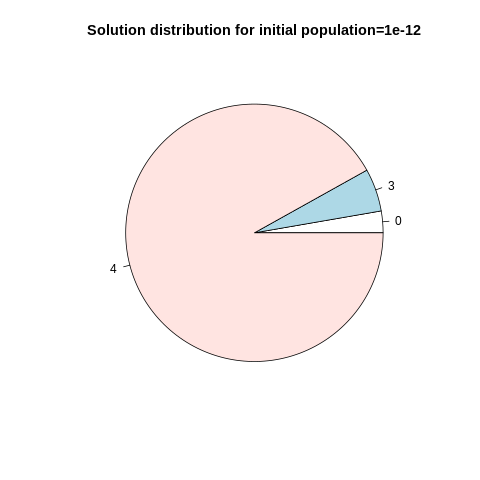
\includegraphics[width=.3\linewidth]{sandbox/graph/1e-12.png}

\end{document}